\chapter{User Guide}
\section{Getting Started and Signing In}
Both Project Managers and Project Members begin on the shared sign-in screen shown below. Once signed in, \textit{SyncFlow} checks your role and takes you straight to the right workspace.

\begin{figure}[H]
    \centering
    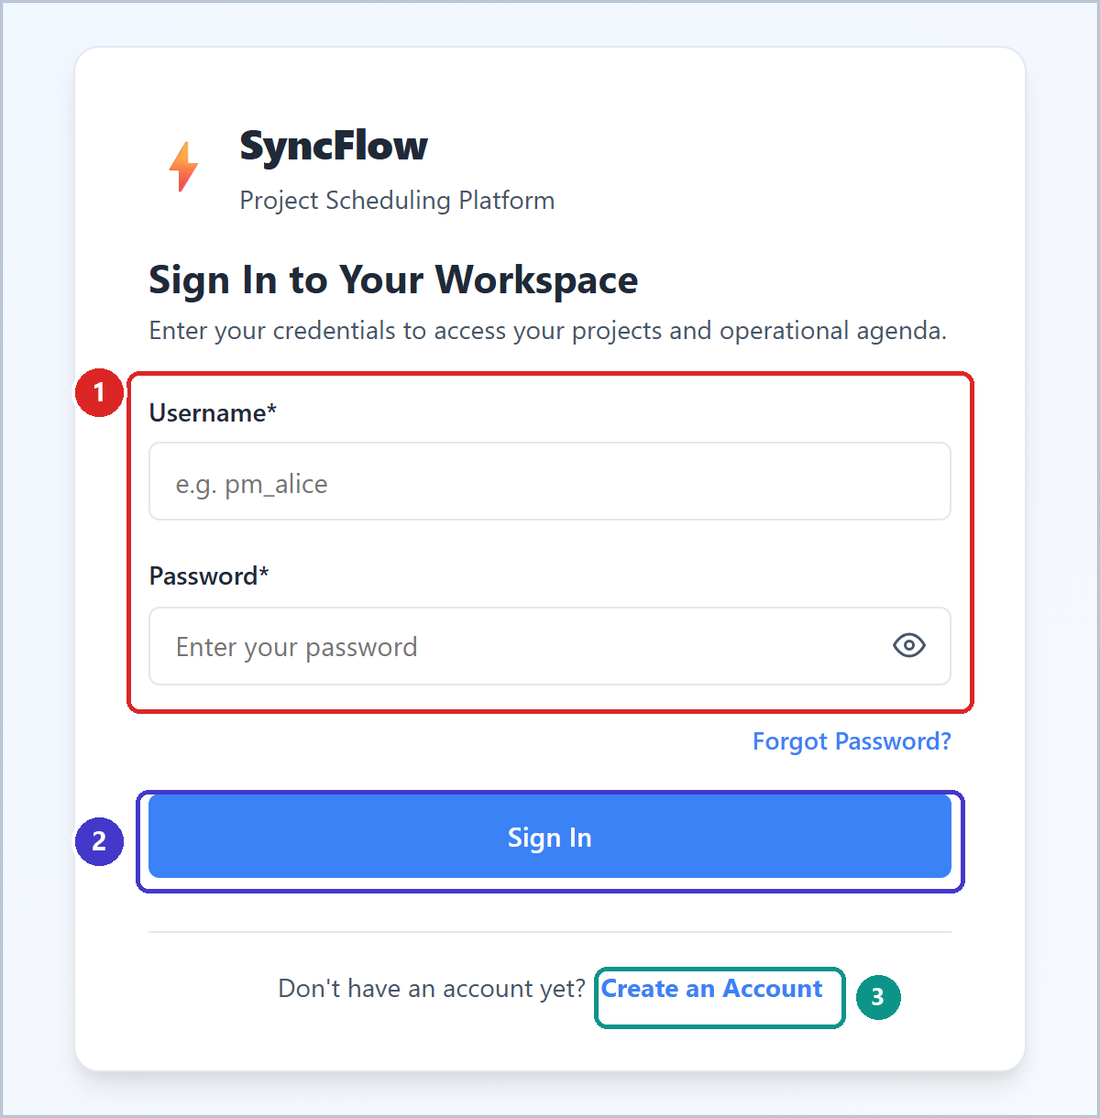
\includegraphics[width=0.41\textwidth]{images/login.png}
    \caption*{SyncFlow sign-in portal with numbered navigation highlights.}
\end{figure}

\begin{enumerate}[leftmargin=2.3em,labelsep=0.6em,itemsep=1pt,topsep=1pt]
    \item \textbf{Account Credentials}: Enter your registered username (or email address) and password. The eye icon lets you double-check what you typed before submitting;
    \item \textbf{Sign In}: Submits your credentials and automatically opens the PM Dashboard for Project Managers or the personal workspace for Team Members;
    \item \textbf{Create an Account}: Opens the registration form for first-time visitors joining \textit{SyncFlow}.
\end{enumerate}

\vspace{2mm}

Clicking \textbf{Create an Account} opens the onboarding form. First, answer the required question asking whether you are a \textbf{Project Manager}: choosing \textit{Yes} unlocks full project creation and scheduling permissions (and sets your role automatically), while choosing \textit{No} creates a standard contributor account where you type your everyday role (for example, Developer or Analyst). Once you pick an option, the remaining fields appear for your first and last name, gender, username, password (entered twice for confirmation), date of birth, email address, and an optional phone number. Submitting the form registers your profile immediately so you can return and sign in.

\vspace{3mm}

If you lose access to your password, click the ``\textbf{Forgot Password?}'' link right above the sign-in button to open the \textbf{Reset Your Password} window. Type either your registered username or email address and press \textbf{Send Reset Link}. \textit{SyncFlow} confirms on screen that recovery instructions have been dispatched for that account, or you can ask a workspace administrator to assist if you cannot access the recovery mailbox.

\newpage

\section{Project Manager Dashboard and New Project Setup}
After signing in, a \textbf{Project Manager} sees the main home dashboard pictured below. From here you can check alerts, review existing projects, or start a new one.

\begin{figure}[H]
    \centering
    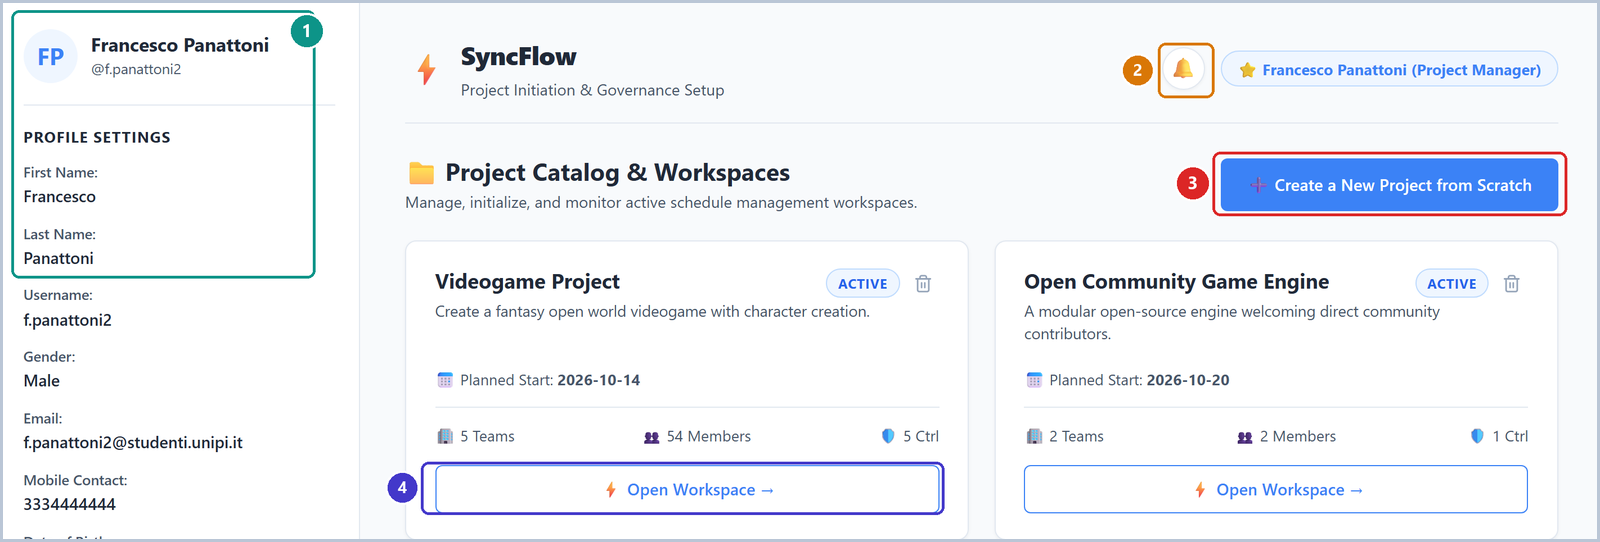
\includegraphics[width=0.85\textwidth]{images/pm_dashboard.png}
    \caption*{Project Manager Dashboard showing project cards, alerts, and workspace entry.}
\end{figure}

\begin{enumerate}[leftmargin=2.3em,labelsep=0.6em,itemsep=1pt,topsep=1pt]
    \item \textbf{Profile Panel}: Displays your name, contact details, and role summary, with buttons to update your details or log out;
    \item \textbf{Notification Bell}: Shows alerts when contributors ask to join a project or submit finished work for review. Join requests can be approved directly from this menu;
    \item \textbf{Create a New Project}: Opens a two-step setup wizard where you name the project, pick its start date, choose whether staff can join multiple teams or request membership openly, and assemble your teams and quality controllers;
    \item \textbf{Project Cards \& Open Workspace}: Each card summarizes team and member counts; clicking \textbf{Open Workspace} opens all six scheduling steps for that project.
\end{enumerate}

In the second step of project creation, shown below, the Project Manager organizes the people who will deliver the work before the project workspace opens. You can build brand-new groups from scratch, copy existing structures via \textbf{Import from Reusable Teams Library}, or list standalone contributors who do not belong to a team.

\begin{figure}[H]
    \centering
    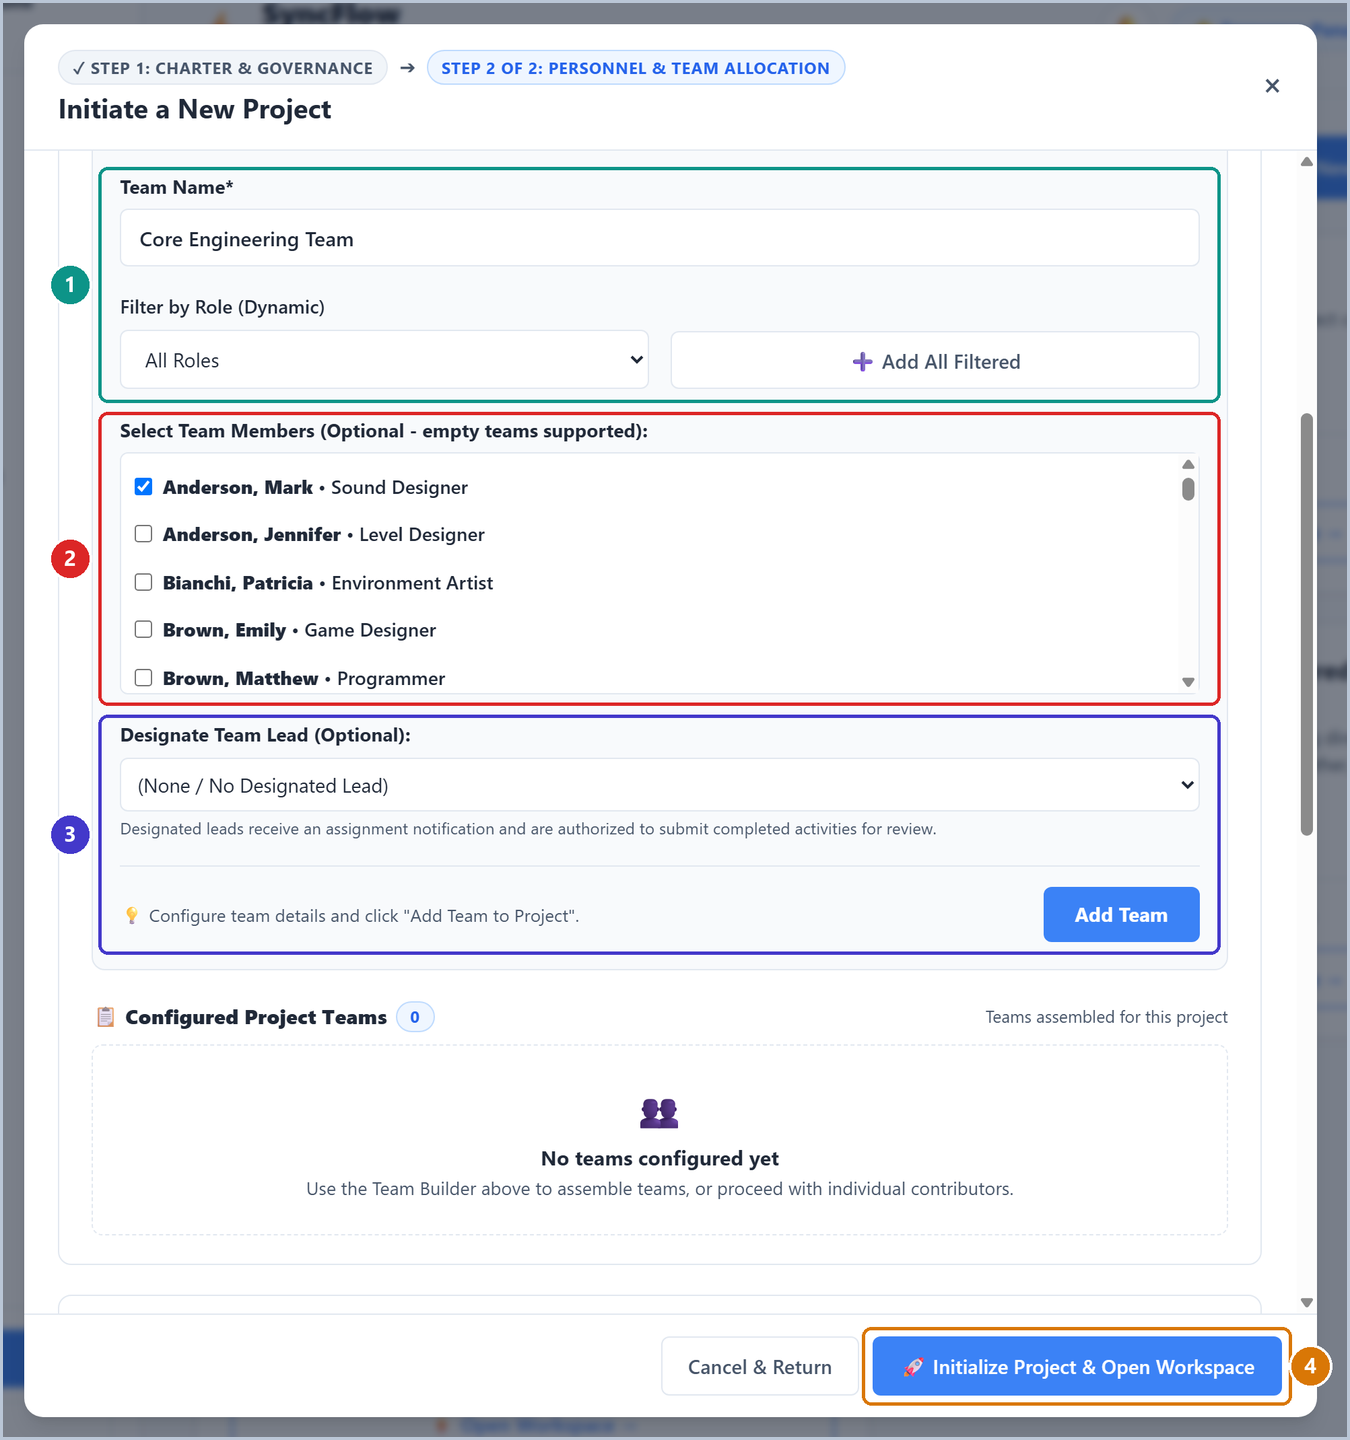
\includegraphics[width=0.5\textwidth]{images/team_allocation.png}
    \caption*{Project creation Step 2 showing team setup, role filtering, Team Lead selection, and launch controls.}
\end{figure}

\newpage

So we have:
\begin{enumerate}[leftmargin=2.3em,labelsep=0.6em,itemsep=1pt,topsep=1pt]
    \item \textbf{Team Name \& Role Filter}: Enter a clear team name, such as \textit{Core Engineering Team}. In larger organizations, use \textbf{Filter by Role (Dynamic)} to narrow down specific specialties and click \textbf{+ Add All Filtered} to add every matching person in one click;
    \item \textbf{Select Team Members}: Tick the checkboxes next to the people you want inside this team. You can also leave everyone unchecked to prepare an empty placeholder team that members can join later;
    \item \textbf{Designate Team Lead \& Add Team}: Optionally choose one selected member as the \textbf{Team Lead} (who receives an assignment notice and is authorized to submit completed activities for review), then click \textbf{Add Team} so the group appears in \textbf{Configured Project Teams};
    \item \textbf{Initialize Project \& Open Workspace}: Repeat as needed for additional teams, optionally select standalone \textbf{Unassigned Individual Contributors} or extra \textbf{Project Controllers} further down the form, and click \textbf{Initialize Project \& Open Workspace} to create the project.
\end{enumerate}

\vspace{4mm}

\section{Planning and Tracking a Project}
\subsection{Manage Personnel (Step 1)}
Inside a project workspace, the left sidebar groups work into six ordered steps matching the schedule lifecycle. Below is how a Project Manager moves through them without needing specialized software training.

\vspace{2mm}

Under \textbf{1. Plan Schedule Management}, you can edit the project goal, review assigned teams, and manage personnel by transferring members between teams, adding staff, or removing them from the project. There are four types of personnel:
\begin{itemize}
	\item \textit{Team members}, who are assigned to a predefined team;
	\item \textit{Individual members}, who work independently (though they may also be assigned to a team);
	\item \textit{Controllers}, who review completed activities, mark them as verified, or provide corrective feedback;
	\item The \textit{Project Manager}, who creates and manages the project and can also act as a controller.
\end{itemize}
For large projects, instead of adding personnel individually, you can create teams and allow members to join them or register independently from a team. 

\vspace{2mm}

\subsection{Breaking the Project into Manageable Pieces (Step 2)}
Before setting dates, big goals are broken down into smaller pieces under \textbf{2. Define Activities}. 

\begin{figure}[H]
    \centering
    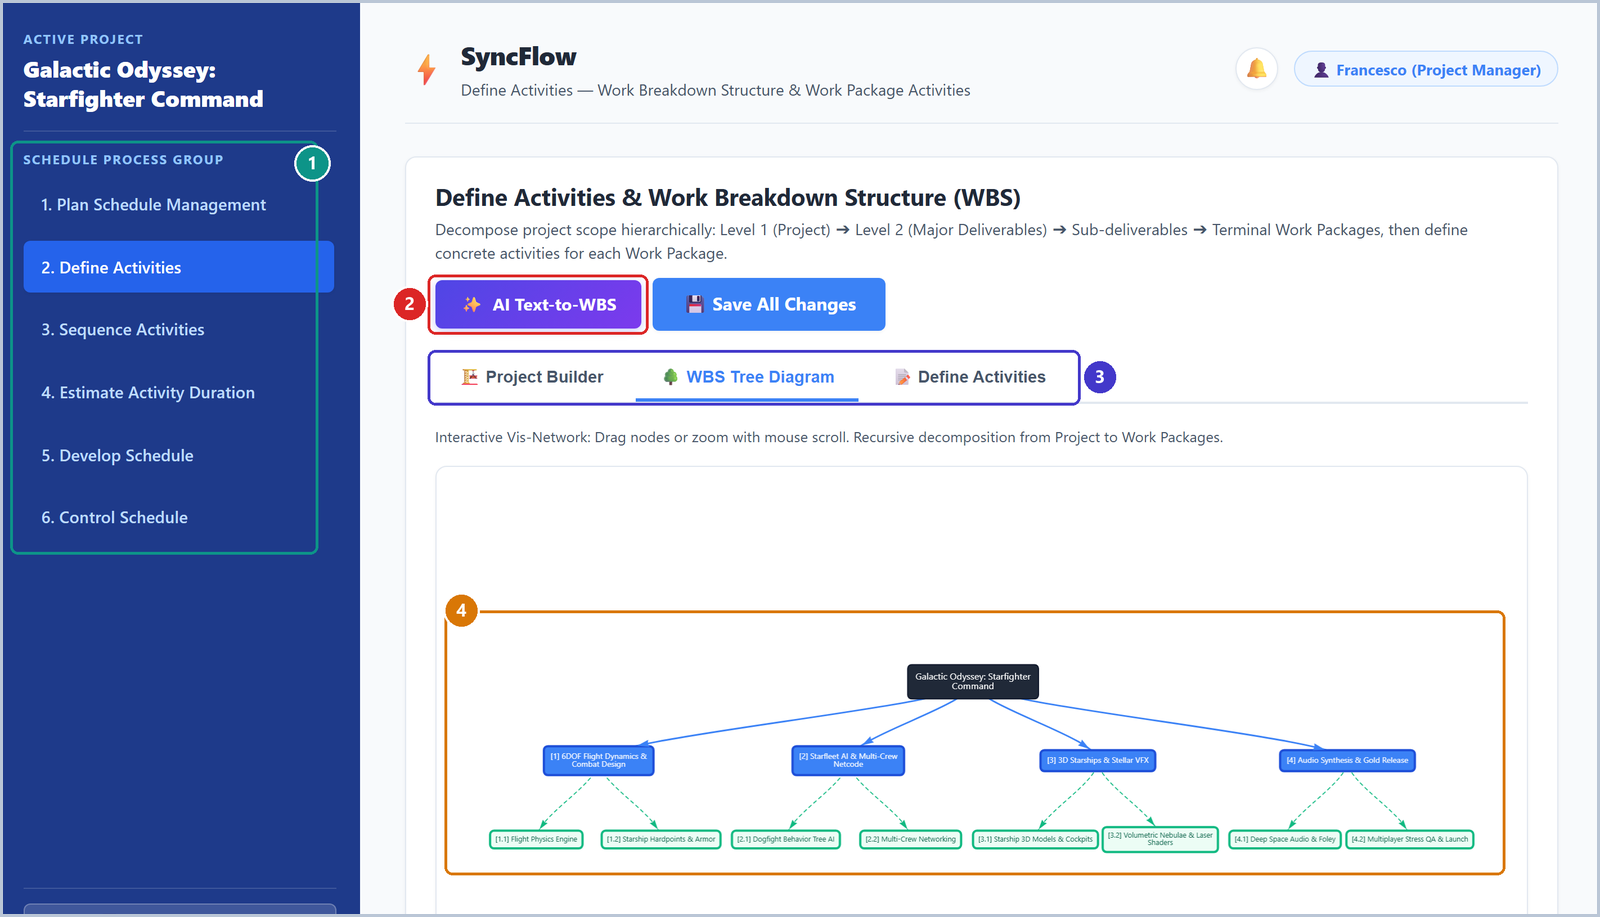
\includegraphics[width=0.50\textwidth]{images/wbs_tree.png}
    \caption*{Define Activities view displaying the interactive Work Breakdown Structure (WBS) tree.}
\end{figure}

\newpage

So we have:
\begin{enumerate}[leftmargin=2.3em,labelsep=0.6em,itemsep=1pt,topsep=1pt]
    \item \textbf{Step Sidebar}: Keeps all six project stages visible on the left so you can jump back to earlier steps at any time;
    \item \textbf{AI Text-to-WBS}: Clicking this purple button lets you paste a plain-text project brief and let the AI draft deliverables, work packages, and activities automatically (choosing either to merge with or replace existing work);
    \item \textbf{Three Sub-Views}: Switch between \textbf{Project Builder} (form cards), \textbf{WBS Tree Diagram} (visual map), and \textbf{Define Activities} (adding work items and zero-day milestones inside each green Work Package);
    \item \textbf{Interactive Tree}: Shows how the project (top box) splits into Major Deliverables (blue) and Work Packages (green).
\end{enumerate}

You do not need the NLP generator to structure a project. Open \textbf{Project Builder} to build the tree manually using nested cards: add \textbf{Major Deliverables}, optional \textbf{Sub-deliverables}, and green \textbf{Work Packages}, renaming or removing items anytime. Then open \textbf{Define Activities}, choose any Work Package, click \textbf{+ Add Activity} to list work items or milestones, and press \textbf{Save All Changes}.

\vspace{4mm}

\subsection{Putting Activities in Order (Step 3)}
Under \textbf{3. Sequence Activities}, you connect work items with arrows so the system knows what has to happen first (shown below).

\begin{figure}[H]
    \centering
    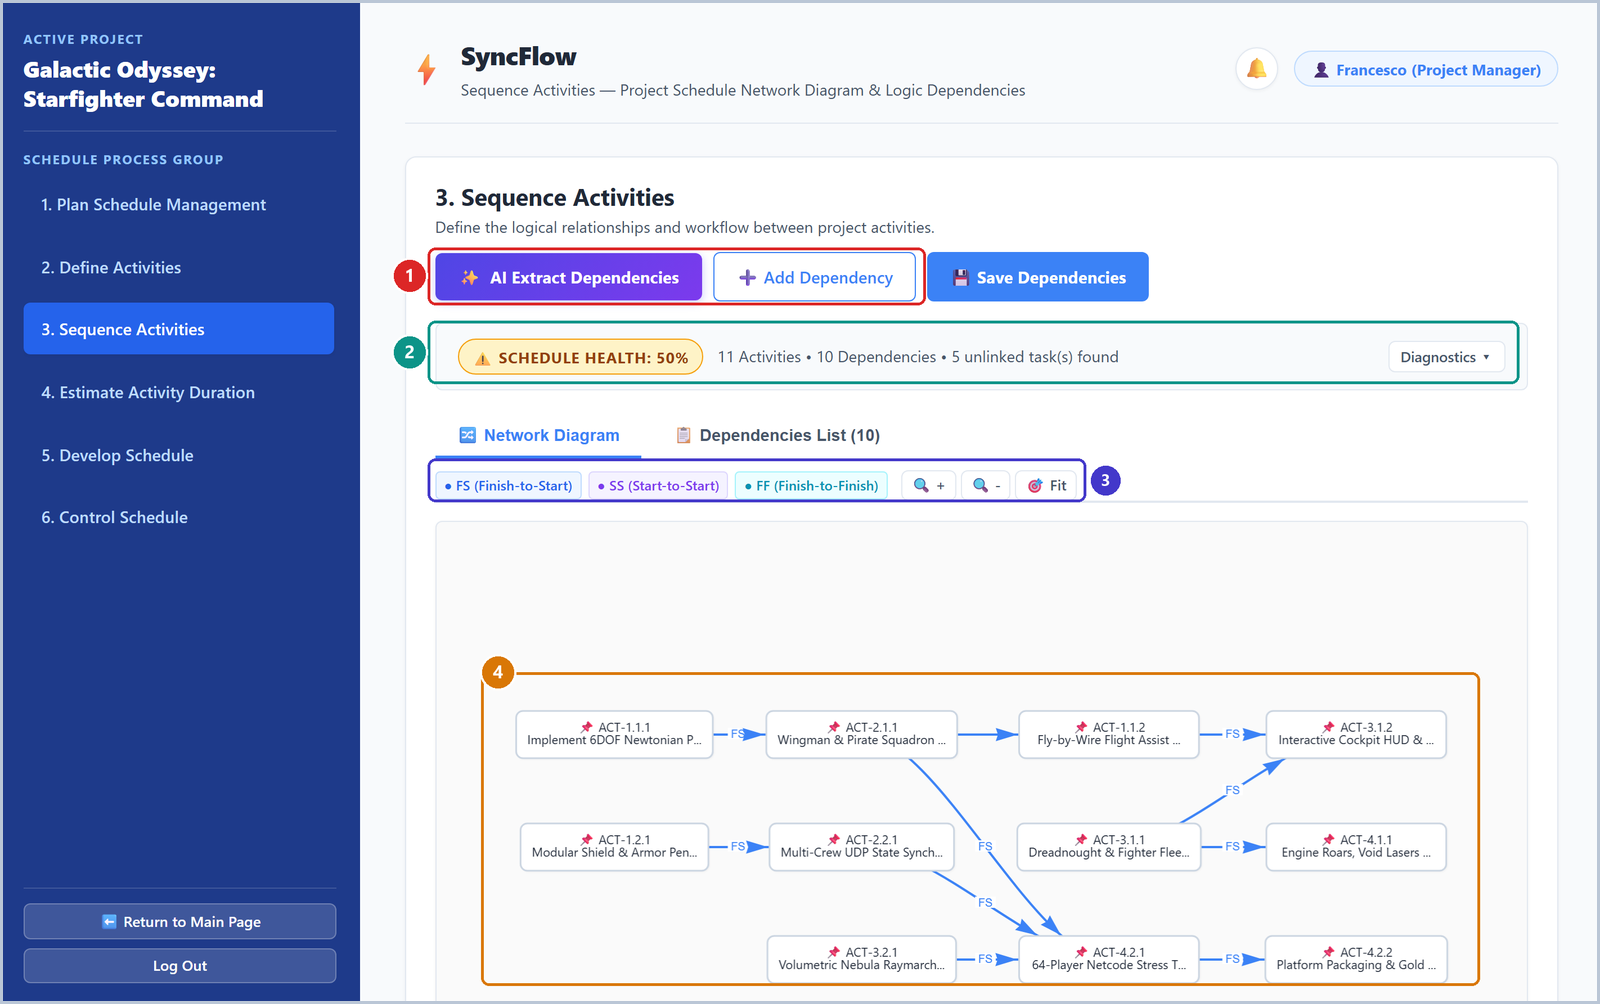
\includegraphics[width=0.8\textwidth]{images/sequence_pdm.png}
    \caption*{Sequence Activities view showing dependency links and health diagnostics.}
\end{figure}

\begin{enumerate}[leftmargin=2.3em,labelsep=0.6em,itemsep=1pt,topsep=1pt]
    \item \textbf{Adding Links Manually or with AI}: Use \textbf{+ Add Dependency} to connect two activities yourself, or click \textbf{AI Extract Dependencies} to read written workflow notes and suggest the connections automatically;
    \item \textbf{Schedule Health Strip}: Flags unlinked items or accidental circular loops right away via the \textbf{Diagnostics} button;
    \item \textbf{Link Legend \& Zoom}: Color tags explain each arrow type (usually \textit{Finish-to-Start}, meaning one job starts after another ends), alongside zoom and fit controls;
    \item \textbf{Network Canvas}: Displays your project flow from left to right so missing handoffs are easy to spot visually.
\end{enumerate}

\newpage

\subsection{Estimating Time (Step 4)}
Under \textbf{4. Estimate Activity Duration}, you estimate how many working days each item will take before \textit{SyncFlow} calculates the full timeline. For each row in the table, you can choose the method that fits best: \textbf{Three-Point (Beta)} asks for best-case, most-likely, and worst-case days so the app balances optimism with risk; \textbf{Single-Point} lets you enter one fixed number; \textbf{Parametric} multiplies work volume by a rate per unit; \textbf{Analogous} lets you reuse the verified duration of a similar activity completed on an earlier project; and \textbf{Milestone} marks a key zero-day checkpoint.

To save time on large schedules, filter controls let you search by name, narrow the list by Work Package or method, or tick \textbf{Show Critical Path Only} to focus purely on items that affect the final finish date, while \textbf{AI DCMA PERT Estimator} can suggest safe ranges automatically. At the top of the screen, a dark \textbf{Target Duration \& Completion Probability Simulator} lets you drag a deadline slider (or pick quick presets such as \textbf{P50}, \textbf{P80}, or \textbf{P90}) to see immediately what percentage chance your team has of finishing by that target day before saving with \textbf{Save Duration Estimates}.

\vspace{4mm}

\subsection{Viewing the Timeline (Step 5)}
\textbf{5. Develop Schedule} turns your dependencies and time estimates into the interactive project calendar shown below. Clicking \textbf{Recalculate Network} refreshes every start date, finish date, and buffer cushion across the project banner.

\begin{figure}[H]
    \centering
    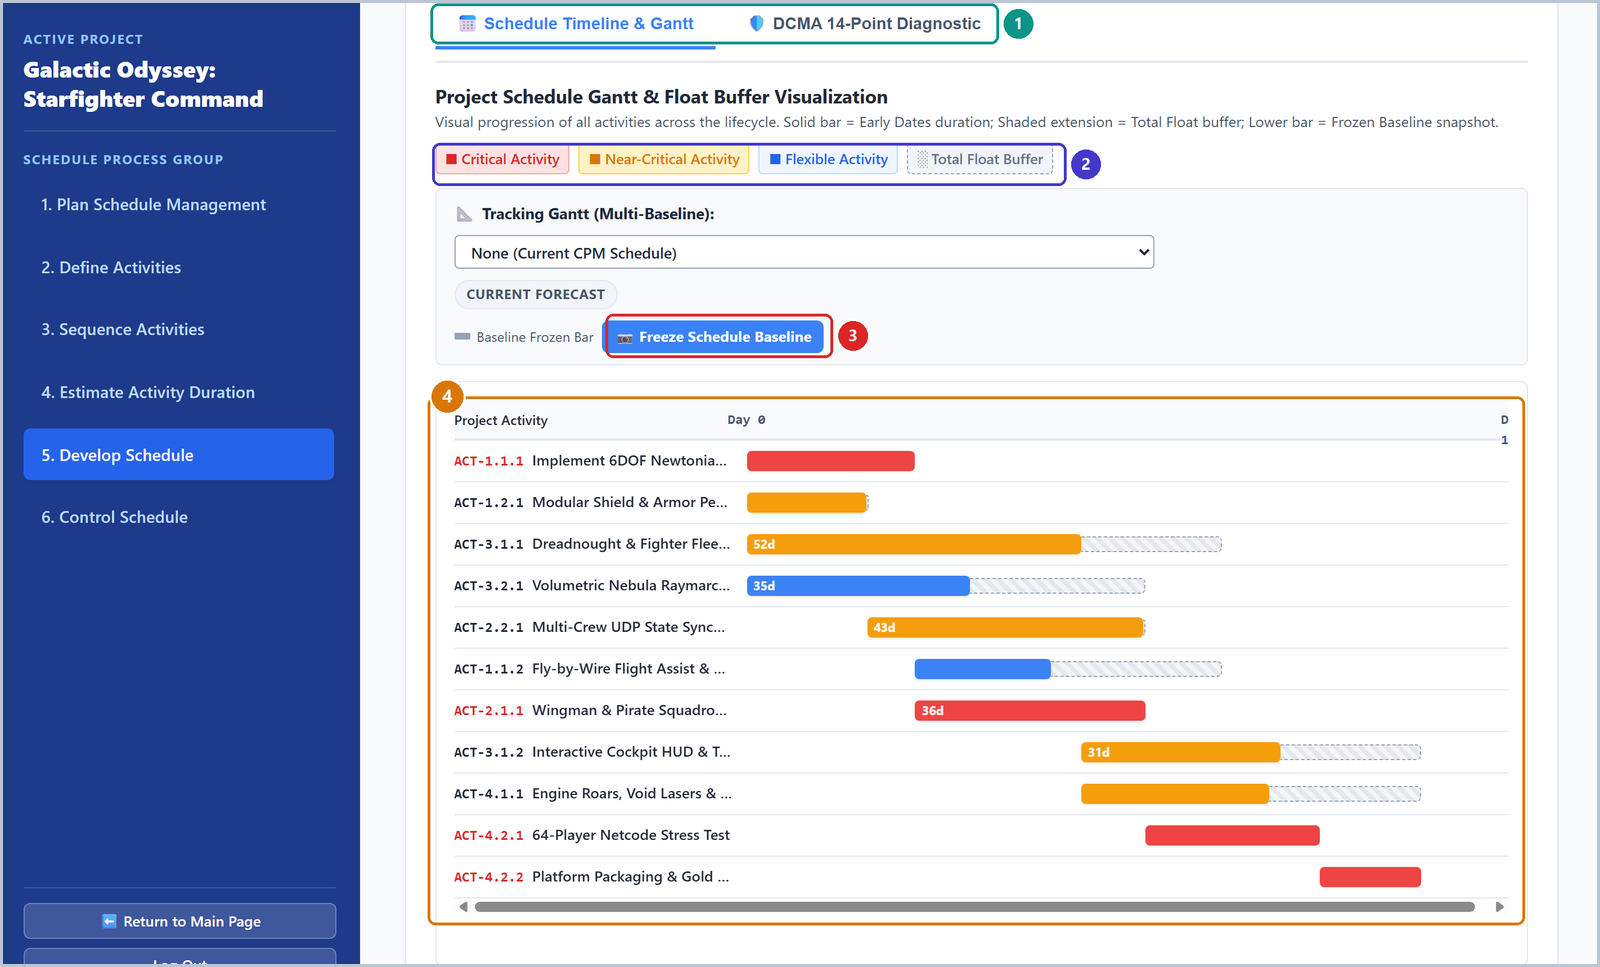
\includegraphics[width=0.78\textwidth]{images/schedule_gantt.png}
    \caption*{Develop Schedule Gantt chart highlighting critical paths, spare buffer days, and baseline locking.}
\end{figure}

\begin{enumerate}[leftmargin=2.3em,labelsep=0.6em,itemsep=1pt,topsep=1pt]
    \item \textbf{Schedule Views \& Quality Check}: Switch across network charts (\textbf{AON} and \textbf{AOA}), float tables, the Gantt timeline, and the automated \textbf{DCMA 14-Point Diagnostic} scorecard;
    \item \textbf{Color Bar Legend}: Red bars mark critical activities (any delay here pushes back the final deadline), amber bars mark near-critical items with tight cushions, and blue bars with gray stripes show spare buffer days;
    \item \textbf{Freeze Schedule Baseline}: Once satisfied with the plan, click this button to lock a saved reference snapshot (or save multiple named baselines) so future delays can be measured cleanly;
    \item \textbf{Interactive Gantt Chart}: Displays start times, lengths, and float cushions across the entire project timeline.
\end{enumerate}

\newpage

Above the chart, the \textbf{Imposed Deadline \& Project Float Manager} lets you enter a client's fixed delivery date so \textit{SyncFlow} shows how many spare \textbf{Project Float} days sit ahead of (or behind) that commitment, while \textbf{Schedule Matrix \& Floats} lists earliest dates, latest dates, and spare buffer days side by side for every item. Meanwhile, the \textbf{DCMA 14-Point Diagnostic} checks the schedule against fourteen common planning pitfalls, grades overall health from A to F, and lists the exact activities that need attention. You can also start the project by clicking a button.

\vspace{4mm}

\subsection{Monitoring Live Progress (Step 6)}
Once the Project Manager clicks \textbf{Start Project}, \textbf{6. Control Schedule} tracks real execution against the frozen baseline (shown below) as of any chosen \textbf{Status Date}. Activities move through four color stages: \textit{Not Started} (gray/white), \textit{Work-in-Progress} (yellow), \textit{Completed awaiting review} (green), and \textit{Verified by Controller} (blue).

\begin{figure}[H]
    \centering
    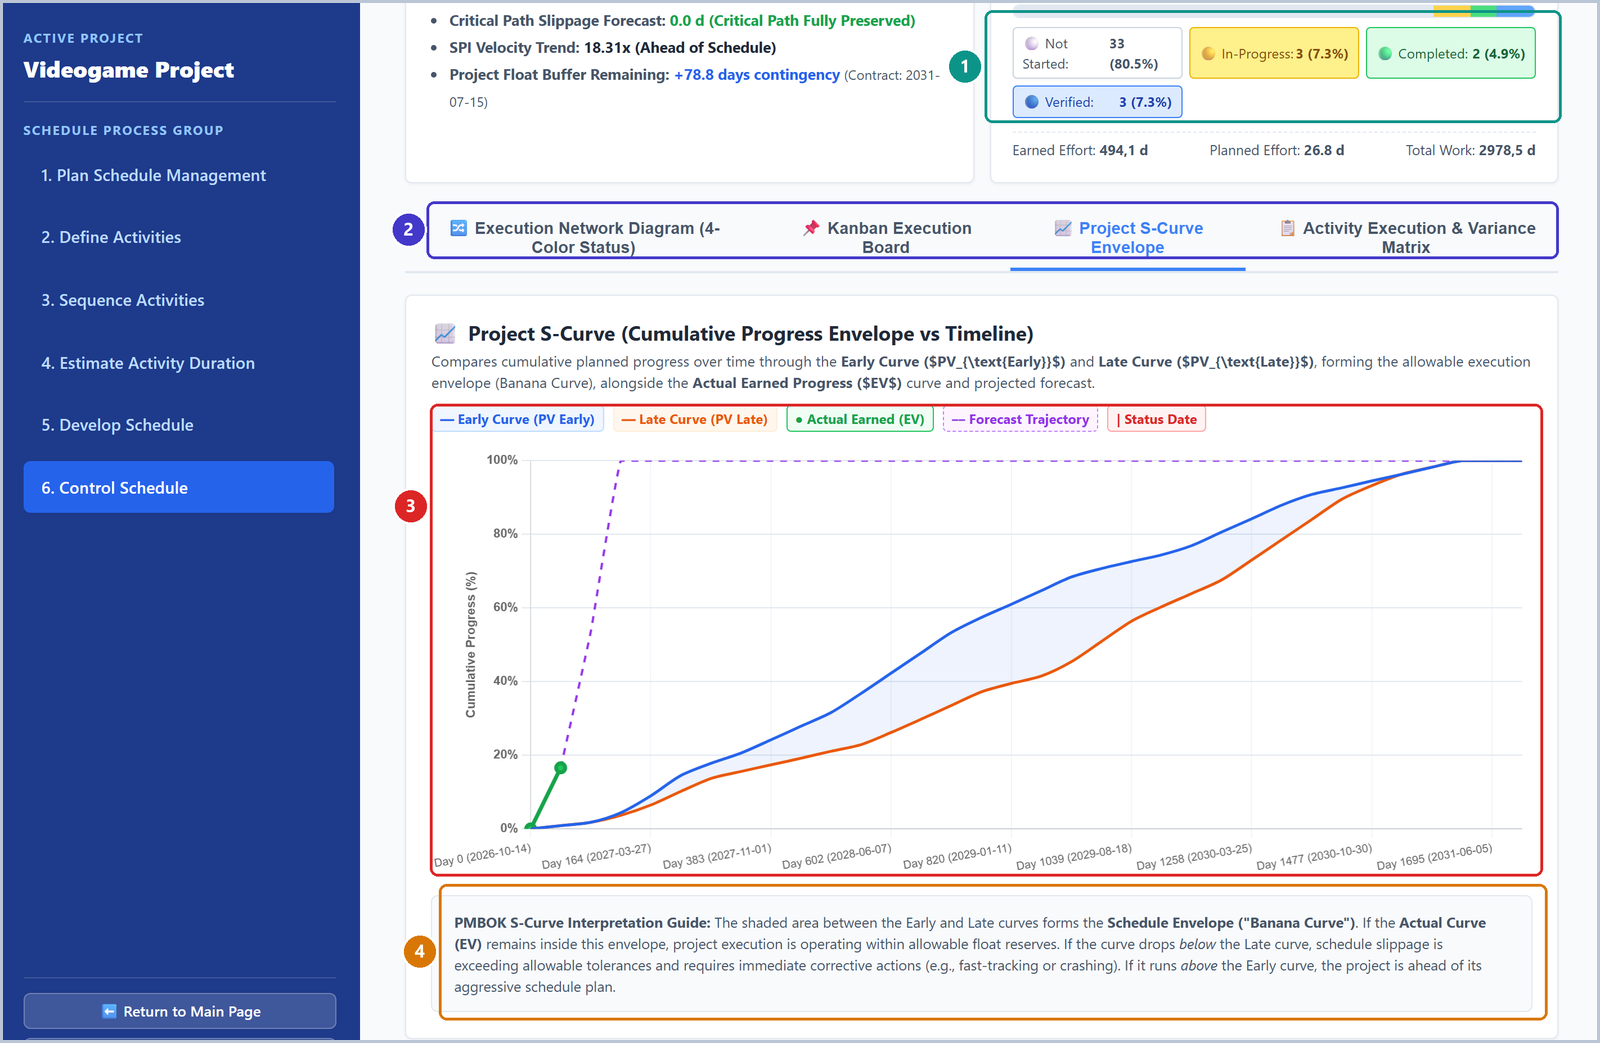
\includegraphics[width=0.78\textwidth]{images/control_scurve.png}
    \caption*{Control Schedule view displaying status totals and the Project S-Curve progress chart.}
\end{figure}

\begin{enumerate}[leftmargin=2.3em,labelsep=0.6em,itemsep=1pt,topsep=1pt]
    \item \textbf{Live Status Breakdown}: Shows how many activities sit in each of the four completion states at a glance alongside earned versus planned work days;
    \item \textbf{Tracking Tabs}: Switch among a 4-color execution network diagram, a four-column \textbf{Kanban Execution Board}, the \textbf{Project S-Curve Envelope}, and a detailed variance table;
    \item \textbf{Progress Chart (S-Curve)}: Compares actual green progress over time against the expected blue and orange planned boundaries. Keeping the green line inside the shaded band means schedule buffers are still holding;
    \item \textbf{Interpretation Guide}: Summarizes in plain text whether work is running ahead of plan, comfortably inside float buffers, or slipping behind schedule.
\end{enumerate}

At the top of the screen, executive summary cards display schedule speed (\textbf{SPI}), time gained or lost (\textbf{SV}), and a projected finish date (\textbf{Forecast Duration}) so delays stand out early. When an activity turns green, a Project Controller (or the Project Manager) opens its review dialog to check submitted evidence and either verify it as blue or return it to yellow work-in-progress with feedback.

\newpage

\section{Daily Workflow for Team Members}
When a contributor signs in, \textit{SyncFlow} hides administrative scheduling menus and opens the personal \textbf{Member Workspace}. Contributors use \textbf{Projects} to revisit teams they already belong to, or open \textbf{Search Projects} to discover new ones across the organization (projects marked open allow instant joining, whereas approval-gated projects notify the Project Manager automatically).

\begin{figure}[H]
    \centering
    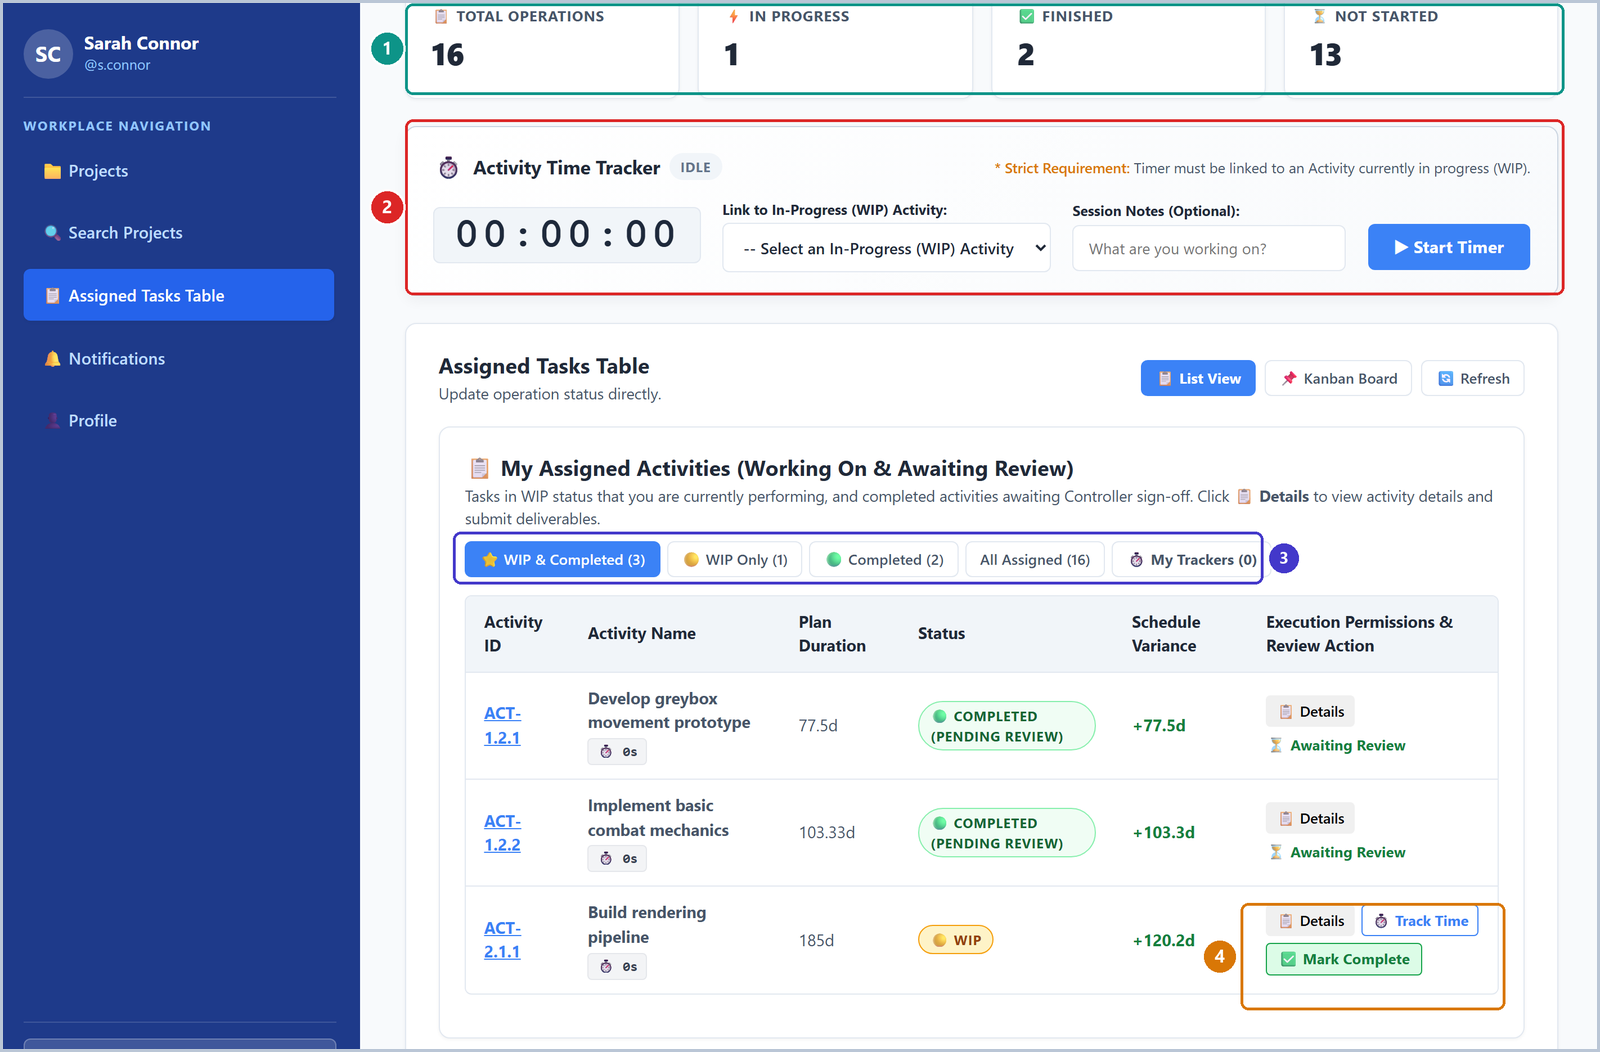
\includegraphics[width=0.77\textwidth]{images/member_workspace.png}
    \caption*{Team Member Workspace featuring the live activity stopwatch and assigned activities table.}
\end{figure}

\begin{enumerate}[leftmargin=2.3em,labelsep=0.6em,itemsep=1pt,topsep=1pt]
    \item \textbf{Work Summary Cards}: Shows live counts of total assigned items, active work in progress, finished deliverables, and not-started assignments for the active project (switchable anytime from the top selector);
    \item \textbf{Activity Time Tracker}: Select an activity currently in \textit{Work-in-Progress (WIP)}, add an optional session note, and click \textbf{Start Timer} to record exact working time without manual spreadsheets;
    \item \textbf{Quick Status Filters}: Filter rows by \textit{WIP \& Completed}, \textit{All Assigned}, or personal tracker logs, or click \textbf{Kanban Board} to work in visual status columns;
    \item \textbf{Action Controls}: Check each row's deadline and schedule variance at a glance, then click \textbf{Track Time} to start logging hours right away, \textbf{Details} to inspect notes and teammate lists, or \textbf{Mark Complete} to submit proof (such as a link or written summary) to a Project Controller for sign-off.
\end{enumerate}

The left sidebar also keeps a permanent \textbf{Notifications} audit log for new project alerts, join approvals, and Controller review notes, along with a \textbf{Profile} section for updating personal contact details and passwords.